\section{Introduction}
Development frameworks based on existing
programming languages and architectural patterns,
have become one of the most
widespread vehicles to create web
applications.
Such frameworks include by default
security features to assist
developers write secure code without
introducing vulnerabilities such as
{\sc sql} injection,
Cross-Site Scripting ({\sc xss}) and
Cross-Site Request Forgery ({\sc csrf}).
In this way,
developers do not have to re-invent the wheel every time they needed to examine
user input or sanitize the output of their
application.

However,
on many occasions developers need
to disable such features to
allow for specific functionalities.
This can re-introduce the
aforementioned vulnerabilities.
In addition,
the complex nature of the
frameworks~\cite{OPM15}
and the various features that they offer
can make the identification of
such defects a difficult task.

{\it Django} is a popular Python-based web
framework that follows the Model
Template View ({\sc mtv}) design pattern,
an adaptation of the
Model View Controller ({\sc mvc})
architectural pattern~\cite{GLH03, BD04}.
In a Django-based application
there is an object-relational mapper
({\sc orm}) that mediates between data models
and a relational database ({\it model}).
There is also a system for
processing {\sc http} requests with
a web templating system ({\it view}),
and a regular-expression-based
{\sc url} dispatcher.
Finally,
both patterns provide several features that
can be used to enhance an application such
as {\it templates} and {\it decorators}.

A potential risk emerges when developers
disable the security checks that the
framework provides,
especially within these features.
In addition,
such issues are difficult to identify because
of inheritance mechanisms supported
by the frameworks,
e.g. a template inherits another one with
disabled security checks.
Notably,
existing mechanisms are not designed
to detect such dangers.

\begin{figure*}[t]
    \begin{center}
        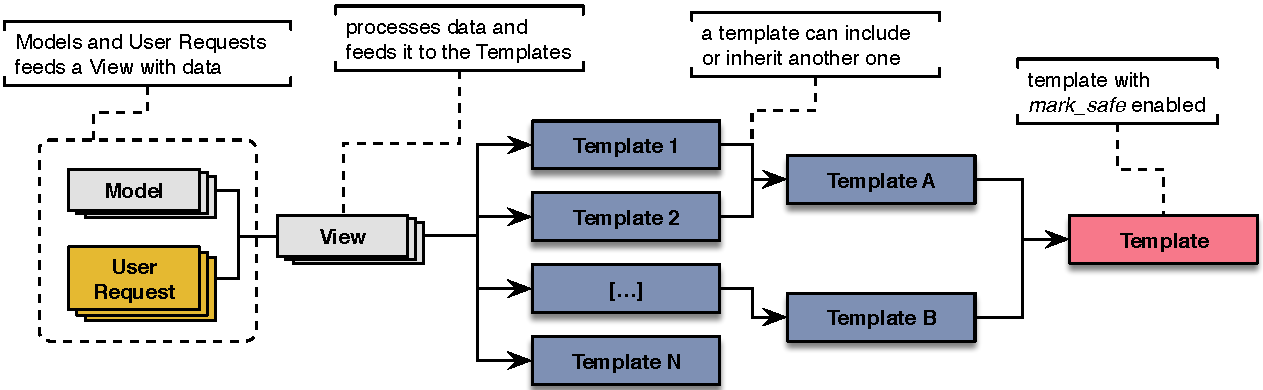
\includegraphics[scale=0.65]{defect_2.pdf}
        \vspace{-2mm}
        \caption{A potentially vulnerable Django
        {\tt template} is included by various templates which in turn are utilized by Django
        {\tt Views}}\label{fig:defect}
    \end{center}
    \vspace{-5mm}
\end{figure*}

To address this issue,
we have developed
{\it Pythia},\footnote{In
ancient Greece, {\it Pythia}
was the name of the high priestess
of the Temple of Apollo at Delphi
who also served as the oracle.}
a mechanism that analyzes
Django-based applications to identify
potentially dangerous data paths.
In particular,
it checks if dangerous code constructs
(i.e. the ones used to bypass the security checks provided by the framework)
are included in an application.
Then,
by performing data-flow analysis
it examines all critical application
parts to identify if any data that
may incorporate user input reaches
the constructs identified in the
first step.
Note that,
Pythia searches for potentially
dangerous data flows.
That is,
an alert does not necessarily involve
an existing hazard.
However,
such alerts can be helpful to
the developer in the future as we
further explain in our ``Evaluation"
section (\ref{sec:eval}).

Our mechanism borrows some of
the standard ideas
(Abstract Syntax Tree ({\sc ast}) analysis)
and terms
({\it sources} and {\it sinks})
of other data-flow
analysis~\cite{LL05, JKK06, DH14}
and taint tracking
schemes~\cite{VFJKKV07, PMP11, SLMS14}
employed to identify
web application defects.
Nevertheless,
it goes one step further and takes
into account the complicated architecture
and the various mechanisms
(inheritance) and features (templates)
of Django-based applications.
To explore paths in such applications
Pythia follows a novel way of
analysis that can be applied
in other similar contexts such
as {\it Laravel}~\cite{laravel},
an {\sc mvc}-based framework used to
create applications in {\sc php}.

We have evaluated Pythia by
examining four,
large,
open-source applications
with thousands of users including
an e-voting service~\cite{zeus-jets},
a cloud service,
and a web-based translation
management system~\cite{weblate}.
In all cases we have identified
corresponding vulnerabilities and
notified the developers.
Apart from the straightforward
{\sc xss} vulnerabilities
(where user input may reach a
sink in a view),
Pythia identified many paths
that involved the particular features of
Django-based applications such as templates.

Three of the applications were patched
hence we provide further details about them.
Following responsible disclosure practices,
we do not reveal the name of
the fourth application and we will
do so once the issue is fixed.

\vspace{-2.5mm}
